\section{API REST}
\label{app:rest}


\begin{table}[H]
\centering
\begin{tabular}{l|l}
\textbf{Endpoint} & \textbf{/rooms}\\
\hline
\textbf{HTPP method} & \textbf{GET}\\
\hline
\textbf{Response Codes} & 
 \begin{tabular}{l|l}
 200 & OK
 \end{tabular}
 \\
\hline
\textbf{Response} & \{"rooms":["Main, ShareLatex, Erlang"]\}\\
\hline

\end{tabular}
\caption{List rooms}
\end{table}


\begin{table}[H]
\centering
\begin{tabular}{l|l}
\hline
\textbf{Endpoint} & \textbf{/room/\{name\}}\\
\hline
\textbf{Parameters} & name - name of the room \\
\hline
\textbf{HTPP method} & \textbf{GET}\\
\hline
\textbf{Response Codes} & 
 \begin{tabular}{l|l}
 200 & OK \\
 404 & If the room does not exist
 \end{tabular}
 \\
\hline
\textbf{Response} & \{"name":"Main","users":["ana", "vitor"]\}\\
\hline

\end{tabular}
\caption{List users in room}
\end{table}


\begin{table}[H]
\centering
\begin{tabular}{l|l}
\hline
\textbf{Endpoint} & \textbf{/room/\{name\}}\\
\hline
\textbf{Parameters} & name - name of the room \\
\hline
\textbf{Headers} & \textbf{Volatile-ChatServer-Auth} - authentication \\
\hline
\textbf{HTPP method} & \textbf{PUT}\\
\hline
\textbf{Response Codes} & 
 \begin{tabular}{l|l}
 201 & Created \\
 401 & Unauthorized \\
 409 & If the room already exits \\
 \end{tabular}
 \\
\hline
\end{tabular}
\caption{Create room}
\end{table}

\begin{table}[H]
\centering
\begin{tabular}{l|l}
\hline
\textbf{Endpoint} & \textbf{/room/\{name\}}\\
\hline
\textbf{Parameters} & name - name of the room \\
\hline
\textbf{Headers} & \textbf{Volatile-ChatServer-Auth} - authentication \\
\hline
\textbf{HTPP method} & \textbf{DELETE}\\
\hline
\textbf{Response Codes} & 
 \begin{tabular}{l|l}
 200 & OK \\
 401 & Unauthorized \\
 404 & If the room does not exist \\
 412 & If the room still has users \\
 \end{tabular}
 \\
\hline
\end{tabular}
\caption{Delete room}
\end{table}


\begin{table}[H]
\centering
\begin{tabular}{l|l}
\textbf{Endpoint} & \textbf{/admin/\{username\}}\\
\hline
\textbf{Parameters} & username - username of the user \\
\hline
\textbf{Headers} & \textbf{Volatile-ChatServer-Auth} - authentication \\
\hline
\textbf{HTPP method} & \textbf{PUT}\\
\hline
\textbf{Response Codes} & 
 \begin{tabular}{l|l}
 201 & Created \\
 401 & Unauthorized \\
 404 & If the user does not exist
 \end{tabular}
 
\hline
\end{tabular}
\caption{Make admin}
\end{table}

\begin{table}[H]
\centering
\begin{tabular}{l|l}
\hline
\textbf{Endpoint} & \textbf{/admin/\{username\}}\\
\hline
\textbf{Parameters} &  username - username of the user \\
\hline
\textbf{Headers} & \textbf{Volatile-ChatServer-Auth} - authentication \\
\hline
\textbf{HTPP method} & \textbf{DELETE}\\
\hline
\textbf{Response Codes} & 
 \begin{tabular}{l|l}
 200 & OK \\
 401 & Unauthorized \\
 404 & If the admin does not exists \\
 \end{tabular}
 \\
\hline
\end{tabular}
\caption{Detailed REST API.}
\end{table}



\section{OrientDB} 
\label{app:orientdb}


\subsubsection{Vertices}\\
\begin{itemize}
\item User: username, password, registrationDate, loggedIn, active;\\
\item Room: name, creationDate, active;\\
\item Message: from, to, text, date.
\end{itemize}


\subsubsection{Edges}\\
\begin{itemize}
\item Messages: from Room to Message: A room has all messages sent in that room linked with an edge; We're not linking the message to the user who sent it because there's no use for that now.\\
\item PrivateMessages: from User who sends to Message and from Message to User who receives: incomings edges are messages receive; Outgoing edges are messages send.\\
\end{itemize}


\begin{figure}
\centering
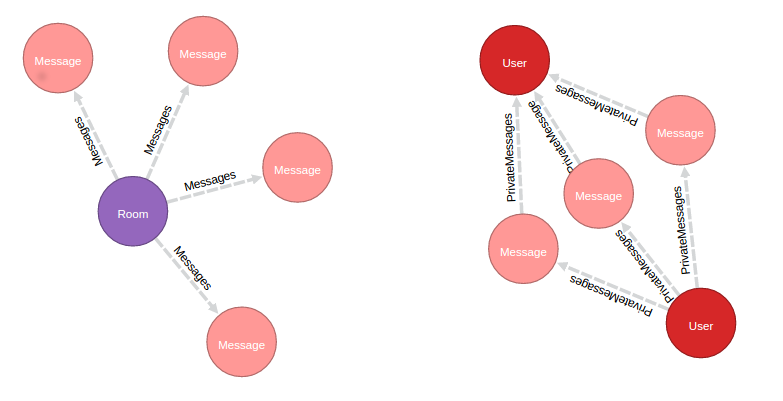
\includegraphics[width=\textwidth]{img/odb_graph.png}
\caption{OrientDB graph example.}
\label{fig:odbgraph}
\end{figure}
